\section{Unifying approaches}
\label{section:inflex:discussion}

In chapter \ref{chapter:preflex}, \ac{PREFLEX} was presented primarily as an architecture for dynamic traffic management, but one in which resilience was identified as a potential benefit given sufficiently adaptive control.
In this chapter, the opposite approach was taken: deriving a traffic management solution from an architecture first built around resilience.

% why INFLEX is better
INFLEX corrected two potential shortcomings in PREFLEX.
Firstly, by eschewing the need for receiver collaboration, INFLEX is unilaterally deployable by edge domains.
Secondly, path acquisition was decoupled from whether a host had timely information on path quality, removing the requirement for flows to incur additional delay on flow start.
As a side-effect, by not tying network processing to SYN packets, INFLEX is also less susceptible to \ac{DoS} attacks.
Nonetheless, INFLEX as presented thus far is geared solely towards resilience.
The remainder of this section details how it can be extended to provide the benefits offered by \ac{PREFLEX}, which are typically of direct interest to operators in particular.

\subsection{Traffic management}

\ac{PREFLEX} offered a fine-grained mechanism for traffic engineering, allowing networks to assign flowlets to network paths.
INFLEX on the other hand only inflects flows upon request. 
This seemingly reduces the opportunities for traffic balancing to when path faults arise.
The host modifications introduced in section \ref{section:inflex:host} however make a provision for flow balancing: on flow start, an INFLEX capable flow has no label associated to the socket, and must consequently acquire whatever label is provided by the edge switch.

% how
Operators can therefore assign flows to specific paths by marking inbound packets with the appropriate label.
Clearly, only the first packet of a flow will take effect -- once a flow has acquired an \ac{INF} label, it will no longer inspect subsequent INFLEX headers unless an inflection request is pending.
As such, one possibility for operators is to intercept the inbound SYN packet and tag it with the appropriate label, in much the same manner as \ac{PREFLEX}.
This presents two challenges.
Firstly, it introduces a \ac{DoS} vulnerability as the amount of network processing is tied to the volume of inbound SYN packets, which can greatly exceed the number of actual flows as shown in figure \ref{fig:flow}.
Secondly, there is no obvious manner of intercepting SYN packets using Openflow as \ac{TCP} flags are not actionable packet header fields.
This means that such functionality would either have to be implemented by specific middleboxes, adding complexity to the proposed architecture, or flow table entries would have to span the entirety of a flow, increasing table size significantly.
In either case, pushing packets to the controller on flow start would necessarily incur a performance penalty for all flows.

A faster, more scalable approach relies on the fact that hosts will ignore the INFLEX header once a label has been acquired.
As such, marking a stream of packets within a flow will have no negative repercussions.
This means that rather than redirecting specific packets to the controller for marking, a rule for marking the inflection label can be installed a priori to the datapath.
Within the flowchart presented in figure \ref{fig:pipeline}, this corresponds to installing a wildcarded entry on the inbound inflection table.
Since such an entry would have a lower priority than pending inflection requests, the basic INFLEX mechanism described in section \ref{section:inflex:arch} remains unaffected.
Since the rule can be wildcarded by network prefix , the number of rules would likely be small. 
Figure \ref{fig:prefix} suggests that over 50\% of traffic is destined to as few as 100 prefixes.
Interestingly, such marking rules need not be applied by the edge switch, instead being performed at a hardware switch relying on \ac{TCAM}.
This both allows larger tables and reduces lookup times, while still delegating policy enforcement to edge switches.

A significant open issue that remains in this regard is how best to dynamically assign flows to routes, as Openflow does not support probabilistic behaviour being pushed to the datapath.
The most obvious approach is to change the mapping between flow and route periodically, in a proportional manner to the desired split.
This raises two potential concerns.
Firstly, flow entries have a time granularity of one second.
While an equal split amongst two paths can be achieved by alternating between flow entries every second, finer flow split ratios over a greater number of paths will incur a much higher periodicity.
Secondly, the impact of this periodicity on overall system behaviour is not clear.
A high path switching frequency may degrade the performance of the switch due to rule churn.
A low frequency on the other hand may induce bursty traffic allocation over short time scales, particularly if flow arrival rates are irregular or the bulk of traffic is composed by short flows.

Under some conditions, a network may need to reassign a flow to another path proactively.
Operators may desire to assign particularly large flows to specific links, clear a link for programmed downtime or allow routing changes to converge before actually using new routes.
In any case, INFLEX provides operators the means to force a path inflection.
This can be achieved in two steps.
The network first clears the INFLEX header for an inbound packet. 
This signals to the end-host that the network is no longer INFLEX capable, leading the network stack to clear the existing \ac{DS} field, as detailed in figure \ref{fig:tcpcode}.
Next, a network sets the INFLEX header for the subsequent packet in the flow.
This leads the receiver to once more adopt INFLEX and acquire the label.
While such forceful behaviour can disrupt transport, it can prove valuable, and networks already have the means to achieve such goals through the cumbersome manipulation of routing.
In this case, INFLEX merely provides existing functionality more flexibly for the network and more transparently for the end-host.

\subsection{Congestion management}

% why previous work still has merit.
One of the unique propositions of \ac{PREFLEX} was to enable networks to perform traffic engineering according to congestion rather than just link load.
This congestion balancing is particularly useful when there is an asymmetry in available bandwidth between providers and when most traffic is not multipath capable.
In order to allow the use of congestion balancing as detailed in chapter \ref{chapter:cate}, INFLEX requires two modifications: hosts must \emph{signal} loss to the network, and the network must \emph{account} for lost packets.

Signalling loss requires marking the outbound INFLEX header.
Given the constraints imposed by the \ac{DS} field, the only option is to reduce the size of the \ac{INF} label to three bits, freeing one bit in the process.
At the transport layer, end-hosts would subsequently set this bit on all retransmissions.
This still allows for seven potential paths per destination, in addition to the default forwarding path.

\begin{figure}
    \centering
    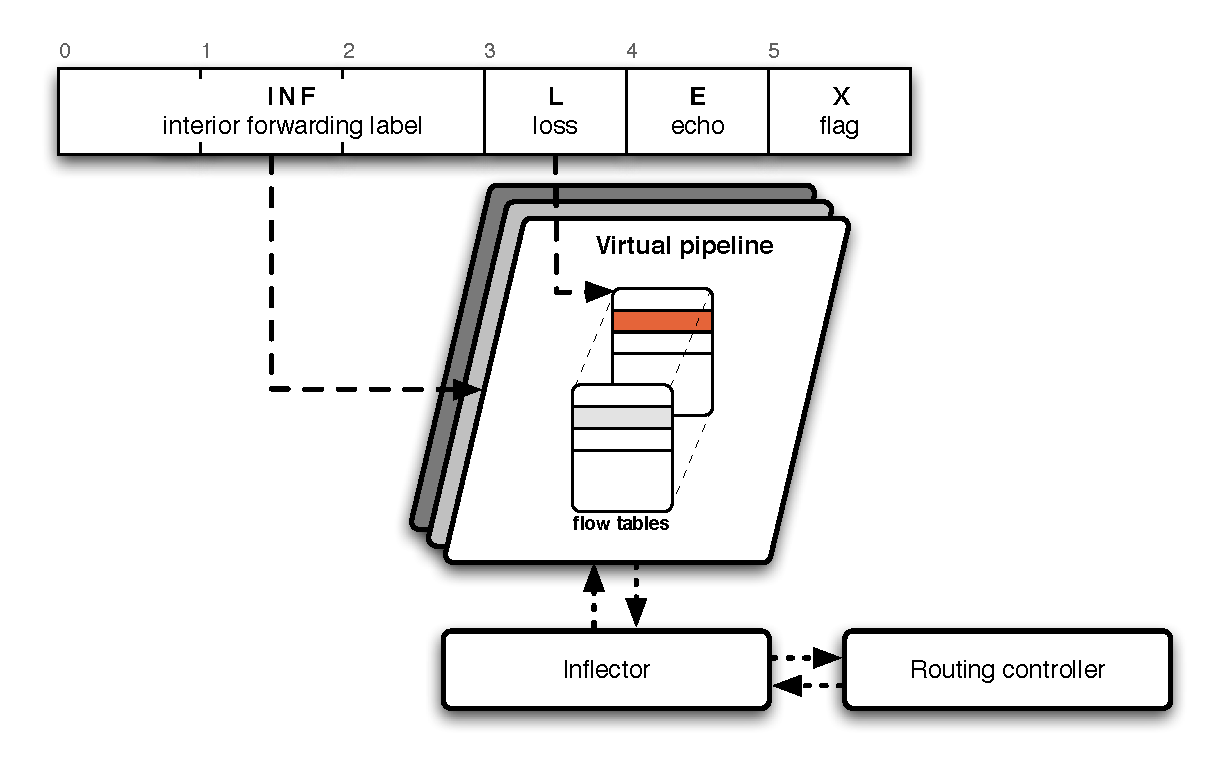
\includegraphics[width=0.7\linewidth]{figures/inflex/infloss}
    \caption[Extending INFLEX for congestion balancing.]{Extending INFLEX for congestion balancing. The \ac{INF} label on outbound packets is used to select the virtual pipeline, while the $loss$ bit is used to toggle between flow tables.\label{fig:inflexloss}}
\end{figure}

% edge switch changes
Figure \ref{fig:inflexloss} displays the resulting header, alongside the changes internal to the network for counting lost packets.
At the edge switch, the datapath remains unchanged, with the \ac{INF} label still being used to select the appropriate virtual pipeline for the outbound packet.
Unfortunately, Openflow does not provide more than one counter per table entry.
Given this constraint, extracting the necessary metrics for performing congestion balancing proceeds by maintaining two replicas of the appropriate routing table.
One flow table is responsible for keeping count of the number of retransmitted packets per entry, while the other accounts for all other packets.
While slightly contrived, this implementation is sufficient for providing congestion balancing as described in chapter \ref{chapter:cate}, and much of the underlying details can be abstracted from the routing controller.

The inflector has the responsibility of exposing an extended Openflow \ac{API} which both implements the routing policies dictated centrally by the routing controller, and returns statistics necessary for route computation.
Whenever a route is \emph{installed} to a given plane, an inflector must insert the corresponding rule into the two parallel flow tables for loss accountability.
Whenever a central controller requests counter metrics for a given entry, the inflector is responsible for returning not only the total number of packets observed for a given route, but also the number of retransmissions.
This cleanly decouples the routing controller from the underlying implementation of INFLEX at the edge switch.
